\documentclass[runningheads]{llncs}

\usepackage{graphicx}
\usepackage{placeins}
\usepackage{flafter}
\usepackage{booktabs}
\usepackage{multirow}
\usepackage{array}
\usepackage{amsmath,amssymb}
\usepackage{url}
\usepackage{microtype}
\emergencystretch=2em
\setlength{\textfloatsep}{8pt plus 2pt minus 2pt}
\setlength{\floatsep}{6pt plus 2pt minus 2pt}
\setlength{\intextsep}{6pt plus 2pt minus 2pt}

% ICISC 2026 anonymous review manuscript.
% Keep author names, affiliations, acknowledgements, grant numbers,
% and identifying repository URLs out of the review version.

\begin{document}

\title{Server-Side Multi-Parent Provenance Reconstruction for Copyright-Related Source Attribution in Heterogeneous Game MOD Packages}
\titlerunning{Multi-Parent Provenance for Copyright-Related Source Attribution}
\author{Anonymous Author(s)}
\authorrunning{Anonymous Author(s)}
\institute{Anonymous Institution}
\maketitle

\begin{abstract}
Game MOD packages contain heterogeneous components such as Java bytecode, structured resources, and images, and may recombine parts of multiple prior MODs, including content from sources absent from the analysis gallery. Copyright-related source review therefore requires technical attribution at component level without assuming that a package has only one source. Pairwise clone detection or whole-package similarity alone cannot simultaneously explain component origins and package-level multi-parent lineage.

To support copyright source attribution, we propose a server-side Hierarchical Multi-Parent Provenance Reconstruction framework that assigns components to registered parents or an open-set \texttt{UNKNOWN} class while reconstructing the package-level parent set. The method extracts identity-neutral content evidence from CODE\_BINARY, STRUCTURED, and IMAGE components without direct identifiers such as paths, project names, or namespaces, then performs global parent retrieval, bounded parent-set inference, and hierarchical component assignment. Dependency topology is limited to an optional refinement inside the candidate set.

Using current and historical releases of real public MOD projects, we construct a 120-project corpus and 540 frozen queries. The final TEST contains 360 queries and 2,520 components across K1, K2, K3, mixed known/unknown, and unknown-only settings. The final method achieves component accuracy 0.805952, \texttt{UNKNOWN} F1 0.753786, and parent-set F1 0.844233. Hierarchical content-only reconstruction improves exact parent-set match from 0.286111 to 0.413889 over independent attribution, whereas the graph-refinement parent-set F1 increment is only +0.000688 and is not statistically conclusive. A FastAPI-based materialized end-to-end pipeline achieves p50 latency of 26.88 ms, and 325 of 489 component errors (66.46\%) occur during component assignment after retrieval.

The system does not automatically determine copyright ownership or infringement. It reconstructs technical provenance between uploaded MOD components and registered reference content to provide evidence for human review of reuse and copyright-related source attribution.

\keywords{Copyright-Related Source Attribution \and Software Provenance \and Game MOD \and Multi-Parent Reconstruction \and Open-Set Attribution \and Software Reuse}
\end{abstract}

\section{Introduction}

Game development and MOD creation frequently reuse code, configuration data, and media assets. Empirical game-software-engineering work documents reuse across code and higher-level assets such as prefabs \cite{trasobares2025reuse}. Direct copying or rebundling may not remain visible in package-manager metadata; software supply-chain frameworks, secure-development guidance, and software-bill-of-materials standards therefore emphasize verifiable artifact provenance and component inventories \cite{torresarias2019intoto,nist2022ssdf,iso5962spdx}. Empirical supply-chain attack research further motivates retaining transformation evidence across package boundaries \cite{ohm2020backstabber}. For copyright-related source review of game MODs, one package may contain Java classes, structured resources, and images from different projects, while some sources may be absent from the server gallery. The technical task is therefore to attribute heterogeneous components, reconstruct multiple registered parents, and retain unexplained content as open-set \texttt{UNKNOWN}.

Clone detection and software composition analysis are strong at code/library reuse but typically return clone pairs or library matches \cite{roy2008nicad,sajnani2016sourcerer,heinze2026stone}. Third-party-library identification extends this analysis to packaged Java/Android and native binaries \cite{backes2016libscout,bincofer2025}. Provenance standards and secure supply-chain research model artifact derivations and transformations \cite{w3c2013provdm,torresarias2019intoto}. We instead study joint component-level registered-parent/\texttt{UNKNOWN} attribution and package-level multi-parent reconstruction for heterogeneous game MOD packages.

We propose Server-Side Hierarchical Multi-Parent Provenance Reconstruction. Identity-neutral CODE\_BINARY, STRUCTURED, and IMAGE evidence is extracted without paths, project names, or namespaces; candidate parents are retrieved globally; and a bounded package-level parent set constrains component assignment. Dependency topology is only an optional refinement. From 120 real public MOD projects and historical releases, we construct 540 frozen queries with project-level calibration, registered TEST, and held-out UNKNOWN splits. On the 360-query TEST, the final method reaches parent-set F1 0.844233 and is additionally evaluated with an external source baseline, a FastAPI server, multi-UNKNOWN stress, retrieval scaling, and failure localization.

Our contributions are:
\begin{enumerate}
    \item an open-set multi-parent formulation for copyright-related attribution of heterogeneous MOD components and package-level lineage;
    \item a hierarchical identity-neutral procedure separating retrieval, parent-set inference, component assignment, and graph refinement;
    \item a frozen real-MOD benchmark with project-level splits, held-out UNKNOWN sources, leakage controls, and exact provenance; and
    \item evaluation of accuracy, uncertainty, ablations, NiCadCross, server latency, multi-UNKNOWN robustness, Exact-versus-LSH scaling, and failure localization.
\end{enumerate}
The output is technical provenance evidence, not an automatic legal determination of copyright ownership or infringement.

\section{Background and Related Work}

\subsection{Code Similarity, Clone Detection, and Software Composition Analysis}
Code similarity spans text, token, AST, graph, and learned representations; established comparisons and a recent systematic review report persistent benchmark, evaluation, and language-support limitations \cite{roy2009comparison,zakeri2023slr}. NiCad uses source normalization for near-miss clones \cite{roy2008nicad}, SourcererCC uses token filtering/indexing at scale \cite{sajnani2016sourcerer}, and transformer-based clone detection has incorporated interpretability \cite{clonexformer2025}. At package/library level, LibScout detects obfuscation-resilient Java/Android libraries \cite{backes2016libscout}, BinCoFer targets partial C/C++ binary TPL reuse \cite{bincofer2025}, and peer-reviewed Android work analyzes obfuscation, versioning, and dependency-fusion challenges \cite{androidtpl2025,libmd2025}. These methods identify reuse but do not jointly reconstruct multiple project parents and an open-set unknown class inside one heterogeneous package.

\subsection{Game-Software Reuse and Copyright-Related Source Review}
Game reuse can combine scripts, prefabs, assets, and scene-related resources, making the practical reuse unit broader than a single source file \cite{trasobares2025reuse}. Software-license audit research further shows that package declarations must be reconciled with file-level artifacts and dependency relations \cite{german2010licensing}. For copyright-related review, we preserve executable, structured, and decoded-image evidence as analyst-facing source evidence rather than a legal determination.

\subsection{Provenance, Lineage, and Multi-Source Reconstruction}
General provenance standards distinguish entities, activities, agents, and derivations \cite{w3c2013provdm}; in-toto records authenticated software-supply-chain steps \cite{torresarias2019intoto}; and ISO/IEC 5962 standardizes SPDX component metadata \cite{iso5962spdx}. These artifact- and metadata-level frameworks complement, but do not perform, the component-level multi-parent reconstruction studied here. Our novelty is not the terms ``heterogeneous provenance'' or ``multi-parent'' themselves, but their concrete combination with component-level registered-parent/\texttt{UNKNOWN} attribution, package-level reconstruction, a frozen real-MOD benchmark, and server-side evaluation.

\section{System and Problem Model}

\subsection{Server-Side Analysis Scenario}

The analysis server maintains previously registered reference MODs. Registration decomposes each package, extracts identity-neutral evidence, and builds a parent-indexed gallery. Online analysis applies the same extractors to an uploaded archive and returns the reconstructed parent set, component labels, and \texttt{UNKNOWN} decisions for human comparison; it makes no legal determination.

\begin{figure}[!htbp]
    \centering
    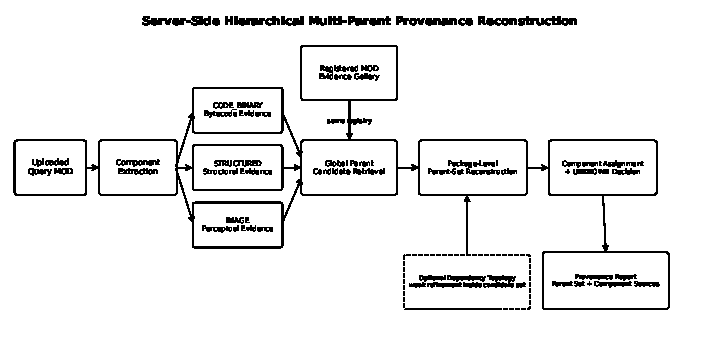
\includegraphics[width=0.90\linewidth]{figures/system_overview_en.pdf}
    \caption{Online provenance reconstruction flow. Identity-neutral content evidence from CODE, STRUCTURED, and IMAGE components is the primary signal; dependency topology is used only as an optional refinement inside the candidate set.}
    \label{fig:system}
\end{figure}
\FloatBarrier

\subsection{Multi-Parent Open-Set Formulation}

Let the registered reference gallery be
\[
\mathcal{G}=\{G_1,\ldots,G_N\}.
\]
A query MOD is represented as
\[
G_q=(V_q,E_q),
\]
where $V_q$ is the component set and $E_q$ is an optional dependency relation. Each component $v\in V_q$ has modality
\[
m(v)\in\{\textsc{Code},\textsc{Structured},\textsc{Image}\},
\]
and provenance label
\[
y_v\in\{1,\ldots,N,\textsc{Unknown}\}.
\]
The package-level registered-parent set is
\[
P_q=\{p\mid \exists v\in V_q,\; y_v=p,\;p\neq\textsc{Unknown}\}.
\]
The system returns component labels $\hat y_v$, a predicted parent set $\hat P_q$, and a registered-parent count $\hat K=|\hat P_q|$.

In this work, \texttt{UNKNOWN} does not mean ``original work'' or ``novel content.'' It only means that the current server-side registered gallery cannot explain the component. Even when multiple distinct unknown sources are present, the primary model exposes a single collapsed \texttt{UNKNOWN} label.

\subsection{Analysis Assumptions and the Hard Evaluation Track}

We do not assume a specific adversarial transformation strategy. Instead, we define a hard evaluation track so that the provenance model cannot rely on easy identity cues such as file paths or naming conventions. The final attribution method does not consume original relative paths, basenames, MOD namespaces, source-project identities, source SHA-256 values, or ground-truth labels. For Java code, the representation also excludes method/class names, descriptors, string constants, and constant-pool operands.

This design prevents trivial solutions that succeed only because names are shared across releases, and forces provenance evidence to come from content structure and behavior-related patterns. It does not imply robustness to every form of obfuscation or semantics-preserving transformation.

\subsection{Structured Objective}

Conceptually, the decision can be written as
\[
\hat{\mathbf y}=\arg\min_{\mathbf y}
\left[
\sum_{v\in V_q}\phi_v(y_v)
+\gamma\Omega(\mathbf y)
+\beta\sum_{(u,v)\in E_q}\psi_{uv}(y_u,y_v)
\right],
\]
where $\phi_v$ is a heterogeneous content-based component-parent assignment cost, $\Omega$ penalizes unnecessary parent proliferation at package level, and $\psi_{uv}$ is an optional dependency-consistency term. In implementation, we avoid direct combinatorial search over the full gallery by separating candidate retrieval from bounded parent-set search.

\section{Proposed Method}

\subsection{Overall Processing Flow}

The proposed method proceeds through seven stages: (1) component extraction, (2) modality-specific identity-neutral evidence extraction, (3) component-to-parent distance computation, (4) package-level candidate retrieval, (5) bounded parent-set reconstruction, (6) component assignment and \texttt{UNKNOWN} rejection, and (7) optional dependency refinement. The central design separates component evidence from package-level decisions. An independent classifier may allow one or two noisy components to introduce additional false parents, whereas the hierarchy first selects a compact parent set using evidence across the entire query.

\subsection{CODE\_BINARY Evidence}

Java class files are parsed into method-level opcode sequences. The identity-neutral CODE representation uses three 128-bit SimHash signatures, following the compact similarity-sketch principle introduced by Charikar \cite{charikar2002simhash}.

First, an opcode 3-gram representation preserves local opcode patterns without operands or constant values. Second, a structural representation summarizes method length, maximum stack, maximum locals, access flags, opcode-category counts, and class-level method/field/instruction counts using log buckets. Third, a context representation uses 3-grams of opcode categories such as arithmetic, branch, load/store, and invoke. This preserves control/operation structure to a limited extent while excluding direct identity information such as class names, method names, descriptors, and string literals.

\subsection{STRUCTURED Evidence}

For JSON-like structured resources, the representation preserves structure and value shape rather than literal identifiers. This follows the reproducibility motivation of canonical JSON representations \cite{rundgren2020jcs}, while the benchmark-specific encoding intentionally retains only identity-neutral structural categories. During key/value traversal, object/array depth, key categories, numeric/string/boolean/null patterns, and sequence structure are converted into tokens and summarized as a 128-bit SimHash. If a resource identifier has the form \texttt{namespace:path}, an external namespace such as \texttt{minecraft} may be retained as a category, while MOD-specific namespace literals are not exposed. Long hexadecimal strings, URLs, and qualified identifiers are likewise mapped to shape categories rather than retained literally.

Trivial structured components that recur across many projects and carry little provenance information, such as empty JSON objects, are removed during benchmark preprocessing.

\subsection{IMAGE Evidence}

IMAGE evidence is computed from decoded pixels rather than file names or paths. We extract 64-bit aHash, dHash, and pHash signatures from grayscale images and compute a normalized 16-bin luminance histogram. Perceptual image hashing is designed to remain stable under visually insignificant transformations \cite{monga2006perceptual}; accordingly, these features can preserve similarity when byte-level SHA changes under lossless re-encoding. IMAGE payloads in the final benchmark are losslessly re-encoded as PNG, and decoded-pixel equality is verified.

\subsection{Component-to-Parent Cost}

Each query component is compared with gallery components of the same modality. Binary signatures use normalized Hamming distance, whereas image histograms use normalized $L_1$ distance. The component distance $d(v,p)$ to parent $p$ is derived from the nearest same-modality evidence owned by that parent.

After normalizing representation-specific distances, we additionally use regret relative to the strongest visible parent. The frozen component cost is conceptually
\[
c(v,p)=\alpha\,\tilde d(v,p)+(1-\alpha)\,\tilde r(v,p),
\]
with $\alpha=0.75$ and regret weight 0.25. Modality-specific open-set thresholds are selected only on the calibration split.

\subsection{Global Candidate Retrieval}

Directly enumerating parent combinations over the entire registered gallery would grow rapidly. We therefore first compute a query-level retrieval score to reduce the search space. For query $q$ and parent $p$, the retrieval score aggregates the $L=3$ smallest component costs:
\[
R_q(p)=\frac{1}{L}\sum_{i=1}^{L}c_{(i)}(p),\qquad L=3,
\]
where $c_{(i)}(p)$ is the $i$th smallest query-component cost for parent $p$. This favors parents supported by several strong provenance signals instead of allowing a single accidental match to dominate ranking. The $M=10$ parents with the smallest $R_q(p)$ are retained as candidate pool $C_q$. On TEST, mean registered-parent recall is 0.974444 and all true registered parents are present for 0.943333 of applicable queries.

\subsection{Hierarchical Parent-Set Reconstruction}

For candidate pool $C_q$, we enumerate parent subsets $S\subseteq C_q$ with $|S|\le K_{\max}=3$. Given $S$, each component chooses the lowest frozen assignment cost among $S\cup\{\textsc{Unknown}\}$. The package objective combines component fit with a parent-count penalty:
\[
J_q(S)=\sum_{v\in V_q}\min_{y\in S\cup\{\textsc{Unknown}\}} c(v,y)+\lambda |S|,
\]
\[
\hat S_q=\arg\min_{S\subseteq C_q,\ |S|\le K_{\max}}J_q(S),\qquad \lambda=0.5.
\]
This hierarchy suppresses the tendency of component-level local optima to introduce too many parents in one query. The final graph variant adds a low-weight boundary-consistency term inside the selected subset, while the content-only variant uses the same candidate pool and package objective without the graph term.

\begin{table}[!htbp]
\centering
\caption{Implementation procedure for Hierarchical Multi-Parent Provenance Reconstruction.}
\label{tab:algorithm}
\scriptsize
\begin{tabular}{p{0.08\linewidth}p{0.84\linewidth}}
\toprule
Step & Procedure\\
\midrule
1 & Extract CODE\_BINARY, STRUCTURED, and IMAGE components from the query package.\\
2 & Compute identity-neutral evidence for each component.\\
3 & Compare with same-modality gallery evidence to compute component-parent costs.\\
4 & Aggregate query-level evidence and retrieve the top $M=10$ registered parents.\\
5 & Evaluate parent subsets with $|S|\le3$ inside the candidate pool.\\
6 & Assign each component to a registered parent or \texttt{UNKNOWN} for each subset.\\
7 & Select the subset minimizing the package objective with parent-count penalty and optional graph term.\\
8 & Return the final parent set, $\hat K$, component labels, and uncertainty-related evidence in the provenance report.\\
\bottomrule
\end{tabular}
\end{table}

\subsection{UNKNOWN Handling}

Open-set thresholds are selected per modality on calibration data and frozen before TEST. The frozen thresholds are 0.1302083284 for CODE, 0.03125 for STRUCTURED, and 0 for IMAGE. The IMAGE threshold of 0 means that this specific frozen representation/calibration selected a highly conservative exact-nearest condition; it is not a universal threshold for other datasets.

The primary TEST contains at most one held-out unknown source per query. A later robustness analysis places two or three distinct held-out donors in the same query to test the stability of collapsed \texttt{UNKNOWN} rejection.

\subsection{Optional Dependency Refinement}

The dependency graph is dominated by Java class references, with sparse non-class edges. We therefore do not describe it as a fully heterogeneous provenance graph. Graph evidence only weakly refines selected-parent assignment within the candidate pool, with frozen weight $\beta=0.1$. The CONNECTED\_STRESS track adds the minimum deterministic bridges needed to connect the five code nodes without using parent labels or $K$, serving as a controlled stress test for cross-parent structural bridges. Consistent with the measured results, the graph is positioned as optional refinement rather than as the central contribution.

\section{Benchmark Construction and Experimental Design}

\subsection{Real MOD Corpus and Historical Releases}

The final corpus contains 120 real public MOD projects: 90 target projects and 30 background projects. For each project, we collect the current release and available historical releases and construct a component registry. Before filtering, the current registry contains 60,257 components and the historical registry contains 178,162 components.

Trivial structured components with little provenance signal, such as empty JSON objects, are removed in advance. After filtering, the current registry contains 56,035 components and the historical registry contains 165,496 components. Cross-project exact-SHA duplicates in the current corpus are limited to five groups covering 48 components. This audit is used to check whether repeated trivial resources could dominate the benchmark.

\subsection{Identity-Leakage Audit}

We analyze identity overlap between 124,470 historical target components and their current releases. Historical components whose exact SHA-256 does not appear in their own current release are defined as hard-masked candidates; 31,279 components satisfy this condition. A stricter subset of 6,429 components also has no identical full relative path in the current release.

Across TEST\_KNOWN historical components, own exact-SHA survival is 0.677471 while same-path survival is 0.919728. This indicates that retaining paths or names would provide a substantially easier identity cue than content transformation. The final method therefore does not use paths, basenames, namespaces, or source-project identities.

\begin{figure}[!htbp]
    \centering
    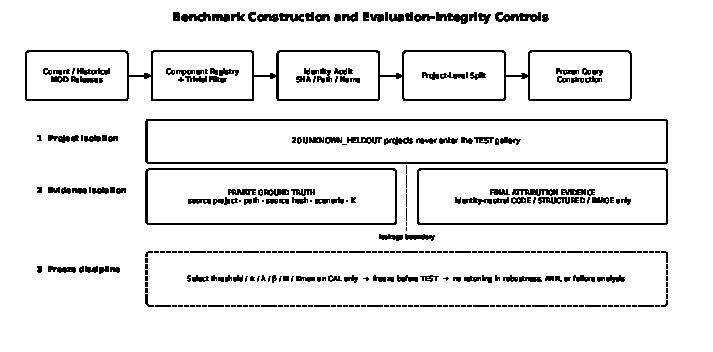
\includegraphics[width=0.88\linewidth]{figures/leakage_freeze_en.pdf}
    \caption{Benchmark construction and evaluation-integrity controls. Project-level open-set isolation, separation of private ground truth from final attribution evidence, CAL-only tuning, and freezing before TEST are enforced together.}
    \label{fig:leakage}
\end{figure}
\FloatBarrier

\subsection{Project Split and Open-Set Isolation}

Project splits are fixed before component-level sampling. This prevents highly similar releases from the same project from appearing in both calibration and TEST.

\begin{table}[!htbp]
\centering
\caption{Frozen project-level split.}
\label{tab:split}
\scriptsize
\begin{tabular}{lrr}
\toprule
Split & Projects & Role\\
\midrule
CAL\_KNOWN & 25 & Registered targets for calibration\\
TEST\_KNOWN & 45 & Registered targets for final TEST\\
UNKNOWN\_HELDOUT & 20 & Open-set sources absent from the gallery\\
CAL\_BACKGROUND & 15 & Calibration-gallery background\\
TEST\_BACKGROUND & 15 & TEST-gallery background\\
\bottomrule
\end{tabular}
\end{table}

The calibration gallery contains 40 projects and the TEST gallery contains 60 projects. None of the 20 UNKNOWN\_HELDOUT projects enters the TEST gallery. After hard masking and fixed-modality-composition constraints, the actual donor pools contain 19 CAL\_KNOWN projects, 33 TEST\_KNOWN projects, and 15 UNKNOWN\_HELDOUT projects.

\subsection{Automatic Query Generation and Ground Truth}

The final benchmark does not rely on manual labels indicating which MOD each file came from. Instead, the historical component registry and a private source manifest automatically select donor projects and source components, and the exact component origin is stored in the private query manifest. Only public/materialized payloads that do not expose source identity are provided to the evaluation pipeline.

A total of 540 queries are generated: 180 for calibration and 360 for TEST. Each query contains exactly seven components:
\[
5\ \textsc{Code}
+
1\ \textsc{Structured}
+
1\ \textsc{Image}.
\]
The complete materialized benchmark therefore contains 3,780 payloads. All 540 IMAGE payloads are losslessly re-encoded as PNG and decoded-pixel equality is verified. Source-hash verification passes for all 3,780 payloads.

TEST contains 60 queries for each of the six scenarios in Table~\ref{tab:scenario}.

\begin{table}[!htbp]
\centering
\caption{Scenario composition of the frozen TEST.}
\label{tab:scenario}
\scriptsize
\begin{tabular}{lrrr}
\toprule
Scenario & Queries & Registered parents & Unknown sources\\
\midrule
TEST\_KNOWN\_K1 & 60 & 1 & 0\\
TEST\_KNOWN\_K2 & 60 & 2 & 0\\
TEST\_KNOWN\_K3 & 60 & 3 & 0\\
TEST\_MIXED\_1K1U & 60 & 1 & 1\\
TEST\_MIXED\_2K1U & 60 & 2 & 1\\
TEST\_UNKNOWN\_K1 & 60 & 0 & 1\\
\bottomrule
\end{tabular}
\end{table}

Using actual total-source count, K=1, K=2, and K=3 each account for 120 queries. The public manifest does not expose K, scenario, source identity, path, or source hash.

\subsection{Graph Track}

For the five selected CODE components, the NATURAL graph preserves historical CLASS\_REF edges. A separate CONNECTED\_STRESS track connects the five code nodes by adding the minimum deterministic bridges without using parent labels or K. This track is not presented as an empirical natural graph; it is a controlled structural stress test of graph-based grouping under cross-parent bridges.

\subsection{Calibration and Freeze Discipline}

All thresholds and reconstruction hyperparameters are selected only on calibration data and are not changed after TEST predictions are observed.

The frozen configuration is: CODE threshold 0.1302083283662796, STRUCTURED threshold 0.03125, IMAGE threshold 0, content weight $\alpha=0.75$, regret weight 0.25, parent penalty $\lambda=0.5$, candidate size $M=10$, graph weight $\beta=0.1$, boundary Top-$R=3$, and $K_{\max}=3$. Later robustness, scalability, and failure analyses do not retune these values.

\subsection{Statistical Analysis and Reproducibility Protocol}

Primary uncertainty is estimated with 10,000 scenario-stratified bootstrap replicates while preserving all seven components of a query as one cluster. Graph-versus-content comparison uses paired bootstrap deltas on the same queries. To examine repeated use of source projects, we additionally perform source-anchor cluster bootstrap and leave-one-source-project-out sensitivity analysis. Parameters are selected on CAL only; TEST is not used for tuning.

When all 2,520 materialized TEST components are re-extracted from raw payloads, every payload SHA-256 matches and all 40,320 compared evidence fields have zero mismatches. Query evidence tables exclude source paths, project IDs, ground-truth labels, scenarios, K, and source hashes, and a programmatic check confirms that UNKNOWN\_HELDOUT projects are absent from the gallery.

\subsection{Experimental Environment}

Primary accuracy evaluation and server benchmarking use the same conceptual pipeline but measure different properties, so their performance values are reported separately. The server host and benchmark protocol are summarized in Table~\ref{tab:environment}.

\begin{table}[!htbp]
\centering
\caption{Server-side benchmark environment and protocol.}
\label{tab:environment}
\scriptsize
\begin{tabular}{p{4.1cm}p{7.1cm}}
\toprule
Item & Configuration\\
\midrule
Host OS & Windows 10, build 26200\\
Python & 3.10.6\\
CPU & 20 physical / 28 logical cores\\
Server & FastAPI / Uvicorn, single process\\
TEST gallery & 60 projects, 26,329 components\\
Concurrency & 1, 4, 8, 16, 32\\
Requests & 200 requests per concurrency level\\
Warm-up & 20 requests\\
Random seed & 20260813\\
Input & Local materialized query ZIP; network upload time excluded\\
\bottomrule
\end{tabular}
\end{table}

The external source baseline uses Open-NiCad/NiCadCross in a WSL Linux environment. StoneDetector is treated as a compatibility audit because the official implementation encounters modern Java bytecode/toolchain issues; we do not over-interpret it as a performance baseline.

\subsection{Metrics and Research Questions}

At component level, we report accuracy and \texttt{UNKNOWN} precision/recall/F1; at package level, parent-set precision/recall/F1, exact match, K accuracy, and K MAE; and at retrieval level, registered-parent recall. Six questions guide evaluation: \textbf{RQ1}, how accurate is copyright-related source reconstruction? \textbf{RQ2}, what do hierarchy and graph refinement contribute? \textbf{RQ3}, how does the method compare with a compatible external clone baseline? \textbf{RQ4}, does the server reproduce frozen decisions with practical performance? \textbf{RQ5}, is it robust to multiple unregistered sources and approximate retrieval? \textbf{RQ6}, where do residual errors arise?

\section{Experimental Results}

\subsection{RQ1: Primary Performance on the Frozen TEST}
\begin{table}[!htbp]
\centering
\caption{Final performance on the frozen primary TEST.}
\label{tab:mainresult}
\scriptsize
\begin{tabular}{lr}
\toprule
Metric & Score\\
\midrule
Component Accuracy & 0.805952\\
UNKNOWN Precision & 0.652427\\
UNKNOWN Recall & 0.892430\\
UNKNOWN F1 & 0.753786\\
Parent-Set F1 & 0.844233\\
Exact Parent-Set Match & 0.419444\\
K Accuracy & 0.486111\\
K MAE & 0.527778\\
Candidate mean registered-parent recall & 0.974444\\
All true registered parents present & 0.943333\\
\bottomrule
\end{tabular}
\end{table}
The final method attains component accuracy 0.805952, \texttt{UNKNOWN} F1 0.753786, and parent-set F1 0.844233. Exact match (0.419444) and K accuracy (0.486111) show that exact source-count recovery remains difficult.

\subsection{Performance by Scenario}
\begin{table}[!htbp]
\centering
\caption{Final results by frozen TEST scenario. Each scenario contains 60 queries.}
\label{tab:scenarioresult}
\scriptsize
\begin{tabular}{lccccc}
\toprule
Scenario & Comp. Acc. & Parent F1 & Exact & K Acc. & UNK F1\\
\midrule
Known K1 & 0.757143 & 0.750000 & 0.283333 & 0.283333 & --\\
Known K2 & 0.809524 & 0.843333 & 0.316667 & 0.383333 & --\\
Known K3 & 0.745238 & 0.787937 & 0.100000 & 0.333333 & --\\
Mixed 1K1U & 0.828571 & 0.930556 & 0.700000 & 0.716667 & 0.847059\\
Mixed 2K1U & 0.797619 & 0.917460 & 0.600000 & 0.683333 & 0.739550\\
UNKNOWN-only & 0.897619 & 0.836111 & 0.516667 & 0.516667 & 0.946048\\
\bottomrule
\end{tabular}
\end{table}
Known K3 has the lowest exact match (0.100000), consistent with the difficulty of recovering all three registered parents simultaneously. Higher mixed-scenario parent-set F1 is interpreted descriptively because source shares differ and unseen sources collapse to one \texttt{UNKNOWN} label.

\subsection{Performance by Modality}
\begin{table}[!htbp]
\centering
\caption{Final component results by modality on the frozen TEST.}
\label{tab:modality}
\scriptsize
\begin{tabular}{lrrrr}
\toprule
Modality & Components & Comp. Acc. & UNK Recall & UNK F1\\
\midrule
CODE\_BINARY & 1,800 & 0.810000 & 0.893773 & 0.766091\\
IMAGE & 360 & 0.972222 & 0.911765 & 0.948980\\
STRUCTURED & 360 & 0.619444 & 0.866667 & 0.581470\\
\bottomrule
\end{tabular}
\end{table}
IMAGE is most stable, CODE\_BINARY is intermediate, and STRUCTURED is hardest. Similar structural shapes after identifier removal motivate stronger structured-resource evidence and modality-specific calibration.

\subsection{Uncertainty: Query Bootstrap and Source-Project Sensitivity}
A 10,000-replicate scenario-stratified query bootstrap gives 95\% intervals [0.787698, 0.823810] for component accuracy, [0.829101, 0.859114] for parent-set F1, [0.372222, 0.466667] for exact match, [0.436111, 0.533333] for K accuracy, and [0.732551, 0.774445] for \texttt{UNKNOWN} F1. Source-anchor bootstrap gives [0.820531, 0.867090] for parent-set F1; leave-one-source-project-out changes remain small (maximum 0.005836 for parent-set F1 and 0.011392 for component accuracy).

\subsection{RQ2: Effect of Hierarchical Reconstruction}
\begin{table}[!htbp]
\centering
\caption{Independent attribution, hierarchical content reconstruction, and final graph refinement.}
\label{tab:ablation}
\scriptsize
\begin{tabular}{lccccc}
\toprule
Method & Comp. Acc. & UNK F1 & Parent F1 & Exact & K Acc.\\
\midrule
Independent & 0.775794 & 0.741806 & 0.797412 & 0.286111 & 0.325000\\
Hierarchical content & 0.807143 & 0.752386 & 0.843545 & 0.413889 & 0.480556\\
Final + graph & 0.805952 & 0.753786 & 0.844233 & 0.419444 & 0.486111\\
Oracle-K content & 0.825794 & 0.790948 & 0.872976 & 0.558333 & 0.627778\\
\bottomrule
\end{tabular}
\end{table}
Hierarchical content-only reconstruction improves component accuracy by +0.031349, parent-set F1 by +0.046133, exact match by +0.127778, and K accuracy by +0.155556 over independent attribution. The graph changes parent-set F1 by only +0.000688 and its paired-bootstrap 95\% interval [-0.001693, 0.003466] includes zero. Oracle-K raises exact match to 0.558333, identifying K inference as a residual bottleneck.

\subsection{RQ3: External Source-Level Baseline}
NiCadCross is evaluated on 1,169 source-resolvable TEST CODE components; 3,275/10,448 gallery CODE components are source-resolvable. With functions/Java/default blind-renaming and threshold 0.30, 10 query and 19 gallery parses fail, yielding 2,199 clone pairs and 505 matched classes.
\begin{table}[!htbp]
\centering
\caption{NiCadCross and the proposed method on the same 1,169 source-resolvable components.}
\label{tab:nicad}
\scriptsize
\begin{tabular}{lccccc}
\toprule
Method & Comp. Acc. & UNK F1 & Parent F1 & Exact & K Acc.\\
\midrule
NiCadCross & 0.710009 & 0.678673 & 0.815468 & 0.725490 & 0.588235\\
Proposed & 0.840890 & 0.794016 & 0.867429 & 0.787582 & 0.771242\\
\bottomrule
\end{tabular}
\end{table}
Paired query-bootstrap intervals favor the proposed method for component accuracy ([0.096187, 0.166524]), \texttt{UNKNOWN} F1 ([0.079256, 0.154288]), and K accuracy ([0.114379, 0.251634]); exact-match delta includes zero. Because NiCad receives reconstructed Java source, this is a same-subset comparison, not a universal-superiority claim. StoneDetector is retained only as a compatibility audit due to modern bytecode/toolchain failures.

\subsection{RQ4: Real Server-Side Evaluation}
\subsubsection{Offline-Server Correctness.}
The single-process FastAPI/Uvicorn server reproduces candidate top-10 results, selected subsets, K, and all 2,520 assignments for all 360/360 frozen TEST queries.

\subsubsection{Materialized End-to-End Latency.}
The benchmark includes archive/manifest parsing, payload reading, raw evidence extraction, 60-project gallery search, reconstruction, graph refinement, and response construction; network upload is excluded.
\begin{table}[!htbp]
\centering
\caption{p50 latency breakdown for a single materialized-package request.}
\label{tab:latency}
\scriptsize
\begin{tabular}{lr}
\toprule
Stage & p50 latency\\
\midrule
Archive open + manifest & 0.334 ms\\
Payload read & 0.232 ms\\
Identity-neutral extraction & 14.440 ms\\
60-project gallery search & 10.685 ms\\
Reconstruction & 1.086 ms\\
Total server processing & 26.880 ms\\
\bottomrule
\end{tabular}
\end{table}
At concurrency 1, total p50 is 26.880 ms; extraction (14.440 ms) and search (10.685 ms) dominate reconstruction (1.086 ms).

\subsubsection{Concurrency and Throughput.}
Across 200 requests at each concurrency 1, 4, 8, 16, and 32, all 1,000 requests succeed. Throughput is 24.72, 37.60, 38.00, 38.71, and 37.16 req/s, peaking at concurrency 16 before single-process contention dominates.

\subsubsection{Real-Project Gallery Scaling.}
Increasing the real gallery from 20 to 100 projects grows components 16,282 to 48,376 (2.97$\times$), search p50 4.353 to 21.457 ms (4.93$\times$), and reconstruction p50 only 0.680 to 1.423 ms. Gallery search is the main scale-up target.

\subsection{RQ5: Multi-UNKNOWN Robustness and Approximate Retrieval}
\subsubsection{Controlled Multi-UNKNOWN Stress.}
A post-freeze 180-query stress test with two or three distinct held-out donors achieves component accuracy 0.841270, \texttt{UNKNOWN} F1 0.887991, collapsed parent-set F1 0.883968, exact match 0.600000, and collapsed K accuracy 0.633333. On 120 queries containing registered parents, registered-parent precision/recall/F1 are 0.815278/0.912500/0.840556 with exact match 0.625000. Rejection remains stable, but unknown identities and multiplicity are not recovered.

\subsubsection{Exact-versus-LSH Retrieval.}
BALANCED and HIGH\_RECALL reproduce all Exact content-only predictions; FAST changes only 1/360 query and 1/2,520 components (component accuracy 0.806746 vs. 0.807143; parent-set F1 0.842804 vs. 0.843545).
\begin{figure}[!htbp]
    \centering
    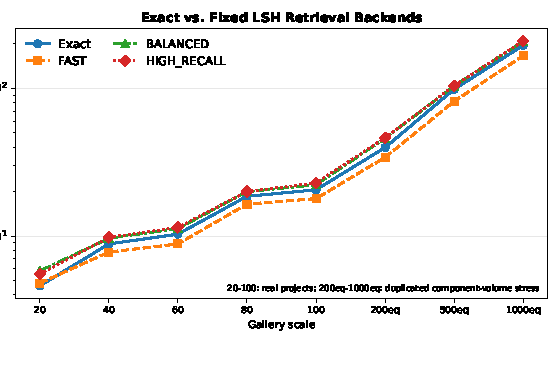
\includegraphics[width=0.80\linewidth]{figures/phase12_scalability_en.pdf}
    \caption{Retrieval p50 for Exact and three fixed LSH configurations. The 20--100 points use real registered-project galleries; 200eq--1000eq are computational component-volume stresses obtained by duplicating arrays from the same 100 real parents.}
    \label{fig:lsh}
\end{figure}
\FloatBarrier
On the 60-project runtime sample, FAST reduces p50 from 10.315 to 8.848 ms (1.166$\times$); fidelity-preserving LSH settings show no p50 advantage over Exact at 20--100 real projects.

\subsection{RQ6: Post-Freeze Failure Localization}
Of 2,520 components, 489 are incorrect: 358 known-to-\texttt{UNKNOWN}, 81 \texttt{UNKNOWN}-to-known, and 50 wrong-known-parent transitions.
\begin{figure}[!htbp]
    \centering
    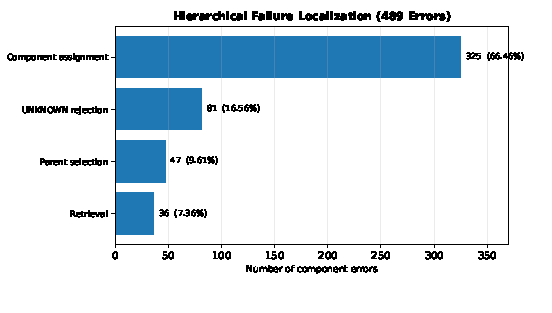
\includegraphics[width=0.70\linewidth]{figures/phase13_failure_breakdown_en.pdf}
    \caption{Hierarchical post-freeze failure localization for all 489 component errors in the frozen TEST.}
    \label{fig:failure}
\end{figure}
\FloatBarrier
Component Assignment Miss dominates with 325 errors, while Retrieval Miss accounts for 36. At query level, 209 parent-set failures split into 192 reconstruction-limited and 17 retrieval-limited cases. All 102 TEST\_KNOWN\_K1 errors are assignment failures; K3 additionally shows 21 retrieval and 19 parent-selection misses. Assignment/\texttt{UNKNOWN} calibration and K inference therefore have higher priority than simply increasing candidate recall.

\section{Discussion}
The ablation identifies hierarchy, not graph refinement, as the main gain: content-only reconstruction improves parent-set F1, exact match, and K accuracy substantially, whereas the graph increment is statistically inconclusive. Of 489 errors, 325 occur after the true parent survives retrieval and package-level selection, and Oracle-K raises exact match from 0.413889 to 0.558333; assignment calibration and source-count inference are thus the main residual bottlenecks. The output remains analyst-facing provenance that narrows candidates and localizes attribution. No score establishes authorship, ownership, copying, permission, license compliance, or infringement, and \texttt{UNKNOWN} only denotes insufficient gallery support.

\section{Limitations and Threats to Validity}
Controlled recomposition yields exact donor labels but does not reproduce all real refactoring, partial edits, image transformations, or resource merges. Because the benchmark is not adjudicated copyright cases, its metrics measure provenance reconstruction, not legal-decision accuracy. Leakage controls remove identity cues and re-extraction shows no mismatch. External validity is limited by the 120-project Java-centered corpus; 200eq--1000eq are computational-volume stresses, not independent real projects. The graph delta is not significant, NiCadCross is source-subset only, and StoneDetector is a compatibility audit. The model exposes one collapsed \texttt{UNKNOWN}, the graph is mainly a Java class-reference backbone, and host-specific latency excludes network upload. Post-freeze analyses do not retune the primary TEST.

\section{Conclusion}
We presented server-side Hierarchical Multi-Parent Provenance Reconstruction for copyright-related source attribution in heterogeneous game MOD packages. From 120 real projects and historical releases, we build 540 frozen queries and 3,780 materialized components; on 360 TEST queries the method achieves component accuracy 0.805952, \texttt{UNKNOWN} F1 0.753786, and parent-set F1 0.844233. Hierarchical reconstruction provides the main gain, while graph improvement is inconclusive. The FastAPI implementation reproduces all frozen outputs at 26.88 ms materialized p50. Future work should prioritize assignment calibration, structured-resource evidence, and source-count inference. The system supports human copyright-related source review, not legal determination.

\begingroup
\renewcommand\small{\fontsize{8}{8.5}\selectfont}
\bibliographystyle{splncs04_unsrt}
\bibliography{references}
\endgroup

\end{document}
